%% 
%% Copyright 2019-2021 Elsevier Ltd
%% 
%% This file is part of the 'CAS Bundle'.
%% --------------------------------------
%% 
%% It may be distributed under the conditions of the LaTeX Project Public
%% License, either version 1.2 of this license or (at your option) any
%% later version.  The latest version of this license is in
%%    http://www.latex-project.org/lppl.txt
%% and version 1.2 or later is part of all distributions of LaTeX
%% version 1999/12/01 or later.
%% 
%% The list of all files belonging to the 'CAS Bundle' is
%% given in the file `manifest.txt'.
%% 
%% Template article for cas-dc documentclass for 
%% double column output.

\documentclass[a4paper,fleqn]{cas-dc}

% If the frontmatter runs over more than one page
% use the longmktitle option.

%\documentclass[a4paper,fleqn,longmktitle]{cas-dc}

%\usepackage[numbers]{natbib}
%\usepackage[authoryear]{natbib}
\usepackage[authoryear,longnamesfirst]{natbib}
\usepackage{glossaries}\usepackage{multirow}
\usepackage{multirow}
\usepackage{subfig}
\usepackage[version=4]{mhchem}
\usepackage{hhline}
%%%Author macros
\def\tsc#1{\csdef{#1}{\textsc{\lowercase{#1}}\xspace}}
\tsc{WGM}
\tsc{QE}
%%%

% Uncomment and use as if needed
%\newtheorem{theorem}{Theorem}
%\newtheorem{lemma}[theorem]{Lemma}
%\newdefinition{rmk}{Remark}
%\newproof{pf}{Proof}
%\newproof{pot}{Proof of Theorem \ref{thm}}

\begin{document}
\let\WriteBookmarks\relax
\def\floatpagepagefraction{1}
\def\textpagefraction{.001}

% Short title
\shorttitle{OpenMC transport independent depletion}    

% Short author
\shortauthors{O. Yardas, P. Romano}  

% Main title of the paper
\title [mode = title]{Extension of the OpenMC depletion module for indirect coupling with external transport solvers}  

% Title footnote mark
% eg: \tnotemark[1]
%\tnotemark[<tnote number>] 

% Title footnote 1.
% eg: \tnotetext[1]{Title footnote text}
%\tnotetext[<tnote number>]{<tnote text>} 

% First author
%
% Options: Use if required
% eg: \author[1,3]{Author Name}[type=editor,
%       style=chinese,
%       auid=000,
%       bioid=1,
%       prefix=Sir,
%       orcid=0000-0000-0000-0000,
%       facebook=<facebook id>,
%       twitter=<twitter id>,
%       linkedin=<linkedin id>,
%       gplus=<gplus id>]

%\author[<aff no>]{<author name>}[<options>]
\author{Oleksandr Yardas}

% Corresponding author indication
\cormark[1]

% Footnote of the first author
\fnmark[1]

% Email id of the first author
\ead{oyardas2@illinois.edu}

% URL of the first author
%\ead[url]{<URL>}

% Credit authorship
% eg: \credit{Conceptualization of this study, Methodology, Software}
\credit{Methodology, Software, Validation, Visualization, Writing - original draft}

% Address/affiliation
\affiliation[1]{organization={Dept. of Nuclear, Plasma, and Radiological Engineering, University of Illinois Urbana-Champaign},
%            addressline={}, 
            city={Urbana},
%          citysep={}, % Uncomment if no comma needed between city and postcode
            postcode={61801}, 
            state={IL},
            country={USA}}

%\author[<aff no>]{<author name>}[<options>]
\author{Paul Romano}

% Footnote of the second author
\fnmark[2]

% Email id of the second author
\ead{promano@anl.gov}

% URL of the second author
%\ead[url]{}

% Credit authorship
\credit{Conceptualization, Methodology, Software, Funding acquisition, Writing - review and editing}

% Address/affiliation
\affiliation[2]{organization={Argonne National Laboratory},
            addressline={9700 S. Ccass Ave}, 
            city={Lemont},
%          citysep={}, % Uncomment if no comma needed between city and postcode
            postcode={60439}, 
            state={IL},
            country={USA}}

% Corresponding author text
\cortext[1]{Corresponding author}

% Footnote text
\fntext[1]{}

% For a title note without a number/mark
%\nonumnote{}

% Here goes the abstract
\begin{abstract}
    We have implemented a new method for running depletion simulations in OpenMC
    that enables indirect coupling to any transport solver. The indirect
    coupling relies on using transport codes to calculate  microscopic cross
    sections. These microscopic cross sections are then used to calculate
    reaction rates, which are used to deplete materials using  
    the existing algorithms in OpenMC's Python API.

    To validate this method, we ran simulations on a simple PWR pincell
    geometry. The new method allows depletion simulations to finish in a matter
    of seconds or minutes. The error for this new method scales with the size of
    the depletion timestep size. For ten 3-day timesteps, fission product errors
    are all under 3\%. Actinide errors range from 10-15\% for \ce{Am} and
    \ce{Cm}, 5-7\% for \ce{Pu} and \ce{Np}, and 2\% and less for \ce{U}. The
    large errors for certain actinides can be attributed to their small
    concentration and difficulty to produce accurately using one-group cross
    sections.

    Our results demonstrates the potential of this new method with moderate
    accuracy and extrodinary time savings for low and medium fidelity
    simulations.
\end{abstract}

% Use if graphical abstract is present
%\begin{graphicalabstract}
%\includegraphics{}
%\end{graphicalabstract}

% Research highlights
\begin{highlights}
\item A new method for running depletion calculations in OpenMC with indirect
    coupling to a transport solver
\item Moderate penalty in accuracy for some actinides for decreased calculation time
\item Low errors for fission products across the board
\end{highlights}

% Keywords
% Each keyword is seperated by \sep
\begin{keywords}
 Depletion \sep Coupling \sep OpenMC \sep Cross sections
\end{keywords}

\newacronym{crpg}{CRPG}{Computational Reactor Physics Group}
\newacronym{ornl}{ORNL}{Oak Ridge National Laboratory}
\newacronym{mit}{MIT}{Massachusets Institute of Technology}
\newacronym{csg}{CSG}{constructive solid geometry}
\newacronym{cfd}{CFD}{computational fluid dynamics}
\newacronym{cad}{CAD}{computer aided design}
\newacronym{dnp}{DNP}{delayed neutron precursor}
\newacronym{ghg}{GHG}{greenhouse gas}
\newacronym{gif}{GIF}{Generation IV International Forum}
\newacronym{msr}{MSR}{molten salt reactor}
\newacronym{msre}{MSRE}{Molten Salt Reactor Experiment}
\newacronym{msbr}{MSBR}{Molten Salt Breeder Reactor}
\newacronym{msfr}{MSFR}{Molten Sodium Fast Reactor}
\newacronym{nrc}{NRC}{Nuclear Regulatory Commission}
\newacronym{rnd}{R\&D}{research and development}
\newacronym{mns}{M\&S}{modeling and simulation}
\newacronym{ent}{E\&T}{education and training}
\newacronym{doene}{DOE-NE}{Department of Energy Office of Nuclear Energy}
\newacronym{cc}{CC}{closed code}
\newacronym{oss}{OSS}{open source software}
\newacronym{iaea}{IAEA}{International Atomic Energy Agency}
\newacronym{oncore}{ONCORE}{Open-source Nuclear COdes for REactor analysis}
\newacronym{snf}{SNF}{spent nuclear fuel}
\newacronym{sfr}{SFR}{sodium-cooled fast reactor}
\newacronym{doe}{DOE}{Department of Energy}

\maketitle

% Main text
\section{Introduction}\label{}
    Modeling and simulation codes will play a critical role in licensing
    advanced nuclear reactors. In preparation for advanced nuclear, both the
    \Gls{doene} and the \Gls{nrc} identified several technical gaps in current
    \Gls{mns} tools that are necessary for efficient and effective license
    application reviews \cite{betzler_modeling_2019} \cite{usnrc_nonlwr_2020-1}.
    The composition of nuclides in a material subject to irradiation over time
    changes due to the nuclear transmutation and decay reactions taking place.
    This process is commonly known as {\it depletion} or {\it burnup}.  Both
    \Gls{doene} and the \Gls{nrc} have specifically identified depletion to be a
    key modeling feature for advanced nuclear reactors.
    
    Modeling depletion in nuclear reactors is inherently linked with modeling
    neutron transport. In order to obtain the transmutation reaction rates
    needed for a depletion calculation, one needs to calculate the neutron flux
    by solving the neutron transport equation. Conversely, after every depletion
    calculation, the transport solution will need  to be run again due the
    change in material composition. This process can be very expensive if
    looking at lifetime behavior of reactor designs, as many transport
    simulations are needed and they must be done sequentially.

    The ExaSMR (Small modular reactor) project seeks to use state-of-the-art
    software tools in Monte Carlo transport and compuitational fluid dynamics
    coupled with heat transfer for simulating advanced reactors along with
    exascale computing hardware to overcome this computational challenge. These
    methods are very computationally expensive, but deliver high confidence in
    their results. If one component in this tool chain could be simplified or
    sped up, it would greatly reduce the computational cost on and economic cost
    from these exascale machines.

    Depletion capabilities were recently added to OpenMC, an open source,
    community developed MC particle transport code \cite{romano_openmc_2015}
    \cite{romano_depletion_2021}. The depletion solver utilizes OpenMC's Python
    API to iteratively run a transport simulation, calculate the reaction rates,
    and update the material composition. In the present work, we describe a new
    method for running depletion calculations without the need to iteratively
    run transport calculations by using precalculated microscopic cross sections
    for each depletion step. At most, only one transport calculation needs to be
    run to generate these cross sections.

    The paper is organized as follows. In Section \ref{sec:methods}, we describe
    the methods and algorithms used to calculate reaction rates using the new
    depletion capabilities. In Section \ref{sec:results}, we describe our
    simulation and analyse the results. In Section \ref{sec:conclusion}, we
    summarize our results, and discuss some gaps in the current implementation
    of the new feature.

\section{Methodology}
    \label{sec:methods}
    We had several design goals for transport-independent depletion functionality:
    \begin{itemize}
        \item Enable use of OpenMC depletion capabilities using only the Python API.
        \item Enable geometry-free depletion
        \item Allow users to pass one or more materials, and specify a power or
            flux along with a set of one-group microscopic cross sections to
            perform depletion.
    \end{itemize}
    
    We created the \verb.IndependentOperator. and \verb.MicroXS. classes to
    achieve these design goals.
    
    \subsection{MicroXS}
        The \verb.MicroXS. class is a subclass of the \verb,pandas.DataFrame,
        indexed by nuclide and reaction name. It also contains methods to create
        a \verb.MicroXS. object by reading a .csv file or a data array. In
        principle, a user could create one-group microscopic cross sections with
        a transport solver code, and then use the \verb.MicroXS. class to read in the
        cross section data for use in depletion. It should be noted that
        \verb.MicroXS. has a function to create one-group microscopic cross
        sections from an OpenMC \verb.Model. object that uses OpenMC's
        \verb.mgxs. module to process tallies.

        We chose one-group cross sections because they are easy to store and
        small, whereas a full continuous-energy cross section library can be on
        the order of gigabytes in size.
        
        Mathematically, calculating reactions rates using one-group cross
        sections should be equivalent to tallying the reaction rates directly.
        In a transport-coupled depletion calculation, reaction rates are tallied
        directly:
        % verify this, I have a suspicion we may need density and volume in there as well
        \begin{equation}
            r^j_i = \int_0^\infty \phi(E) \sigma^j_i(E) dE
        \end{equation}
        where $i$ and $j$ indicate the nuclide and reaction, respectively.

        These reaction rates are in units of reactions/src particle, so we need
        a normalization factor $f$ in src/s to get reactions/s:
        \begin{equation}
            R^j_i = r^j_i * f
        \end{equation}

        In obtaining one-group cross sections for a transport-independent
        depletion, we would also compute $r^j_i$ from a transport calculaton, as
        well as the energy-averaged flux (in units of particle-cm / src):
        \begin{equation}
            \bar{\phi} = \int_0^\infty \phi(E) dE
        \end{equation}
        and then compute the one-group macroscopic cross section:
        \begin{equation}
            \bar{\Sigma}^j_i = \frac{r^j_i}{\bar{\phi}}
        \end{equation}
        Notice that the src unit cancels out, leaving us with $cm^{-1}$, which
        are indeed the correct units.

        When we go to compute reaction rates, we use the equation 

        \begin{equation}
            R^j_i = \bar{\phi'} \bar\Sigma^j_i = r^j_i\frac{\bar{\phi'}}{\bar{\phi}} = r^j_i f
        \end{equation}
        where $\bar{\phi'}$ is the `true' neutron flux. By inspection, we can
        see that $f$ has the correct units of src/s. It follows that using a
        single energy group and energy-averaged flux to calculate reaction rates
        is mathematically equivalent to the statistical tallying of reaction
        rates.

            
    \subsection{IndependentOperator}
        The \verb.IndependentOperator. class uses an instance of the
        \verb.MicroXS. class to calculate the reaction rates using one-group
        microscopic cross sections via the following equation:
        \begin{equation}
            R^j_i = \bar{\phi'} \bar{\sigma}^j_i n_i V
        \end{equation}
        where $\sigma$ is the microscopic cross section, $n$ is the number
        density [$at/cm^3$] and $V$ is the volume [$cm^3$]. The microscopic
        cross sections are stored in a \verb.MicroXS. object which must be
        provided the user. This opens up indirect coupling to any transport code
        that can calculate one-group microscopic cross-sections. After some
        slight modifications to the existing OpenMC API, only these two classes
        are needed to perform transport independent depletion.

\section{Results}\label{sec:results}
    To validate this new feature, we performed a parameter scan study on a PWR
    pincell geometry.  Table \ref{tab:mat-params} contains the material
    parameters of our model, and Table \ref{tab:geo-params} contains the
    geometric parameters.

    We used the ENDF/B-VII.1 nuclear data library available at
    \url{openmc.org/official-data-libraries}. We used the ENDF/B-VII.1 depletion
    chain in the PWR spectrum available at \url{openmc.org/depletion-chains}.
    
    \begin{table}
        \caption{Material Parameters}\label{tab:mat-params}
        \begin{tabular*}{\tblwidth}{|c|c|c|c|}
            \hline
             Item & Fuel & Cladding & Water \\ % Table header row
            \hline
             Density [g/cc] & 10.4 & 6 & 1.0\\
             Volume [cc] & 0.1764$\pi$ & & \\
             S($\alpha$,$\beta$) &  & & \verb.c_H_in_H2O.\\
            \hline
        \end{tabular*}
    \end{table}
    
    \begin{table}[<options>]
        \caption{Geometric Parameters}\label{tab:geo-params}
        \begin{tabular*}{\tblwidth}{|c|c|c|}
            \hline
            Fuel Radius & Clad Radius & Water Bounding Box dimensions\\
            \hline
            0.42 & 0.45 &  1.24 $\times$ 1.24\\
            \hline
        \end{tabular*}
    \end{table}


    We used timestep size, depletion timestepper, and normalization method as
    our parameters to vary.

    Table \ref{tab:timestep-shorthands} shows the different timestep sizes we
    used and their shorthand terminology. All simulations ran for 10 depletion
    steps.

    \begin{table}[<options>]
        \caption{}\label{tab:timestep-shorthands}
        \begin{tabular*}{\tblwidth}{@{}LL@{}}
            \toprule
            Timestep sizes & Shorthand term \\ % Table header row
            \midrule
            360 seconds & Minutes\\
            4 hours & Hours\\
            3 days & Days\\
            30 days & Months\\
            \bottomrule
        \end{tabular*}
    \end{table}
    
    We used two different depletion timesteppers: \verb.PredictorIntegrator.,
    analagous to Gauss' method, and \verb.CECMIntegrator., a predcitor-corrector
    extension of Gauss' method.

    The last parameter, determines how neutron flux is calculated, and we also
    had two values for this: \verb.fission-q. normalization, and
    \verb.source-rate. normalization. \verb.fission-q. normalization uses
    fission Q  values in the depletion chain to calculate the flux. For the
    \verb.IndependentOperator. class, the equation used to calculate the flux
    using fission Q values is

    \begin{equation}
        \bar{\phi'} = \frac{P}{\sum\limits_i (Q_i \bar{\sigma}^f_i N_i)}
    \end{equation}

    where $P$ is the power, $Q_i$ is the fission Q value for nuclide $i$,
    $\bar{\sigma}_i^f$ is the one-group microscopic fission cross section for
    nuclide $i$, and $N_i$ is the number of atoms of nuclide $i$.

    \verb.source-rate. normalization uses a constant flux value to calculate the
    reaction rates. We caclulated the flux based on the initial material
    composition of the PWR pincell to be 1164719970082145.0 n/cm$^2$-s

    For each parameter combination, we ran with three cases:
    \begin{enumerate}
        \item Transport-coupled depletion
        \item Transport-independent depletion
        \item Transport-independent depletion with microscopic cross sections
            updated after each depletion step.
    \end{enumerate}

    For the first case, we used 25 inactive and 125 active batches, with 1e6
    particles per batch.

    We wrote a custom script to run the the third case. It should be noted that
    the third case is significantly slower than using transport-coupled depletion
    as the cross sections need to be reloaded after each depletion step due to how
    we wrote the script.

    Three cases and 16 parameter combinations gives 48 simulations total. All
    depletion simulations used a linear power density of 174 W/cm.

    To avoid a prohibitvely long paper, we will only show a subset of the
    results for each parameter. Unless otherwise specified, all results are
    using 3 day timesteps, \verb.fission-q. normalization, and
    \verb.PredictorIntegrator.  The general trend is that errors are smaller for
    shorter depletion timesteps, and larger for longer depletion timesteps.
    Interested readers can find the full results -- including figure geneartion
    scripts for all cases --  \ldots

    %TODO: Get the external data repo set up!!

    % actinides error 

    \begin{figure}[h!tpb]
        \centering
        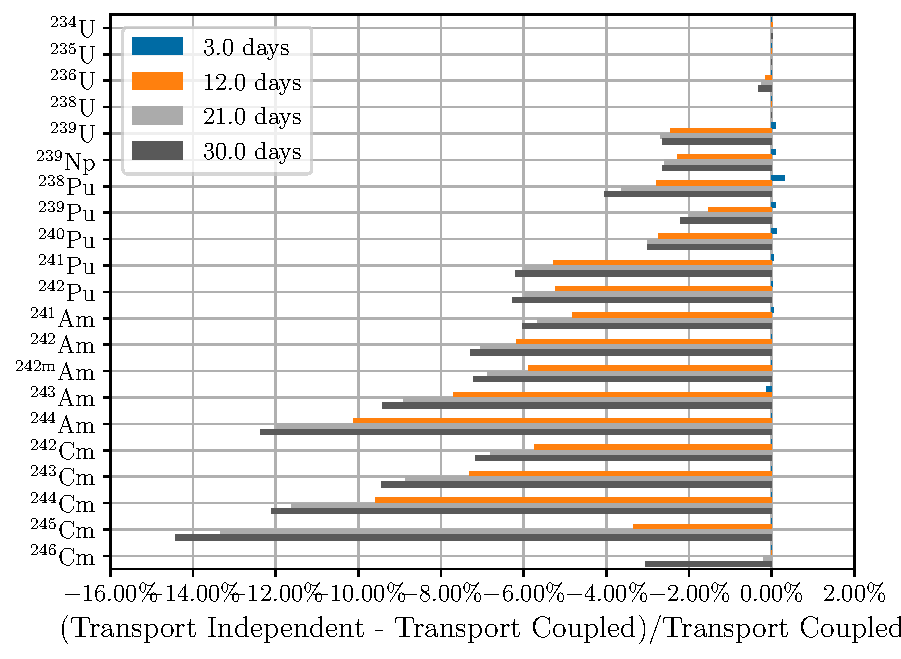
\includegraphics[width=\linewidth]{figs/actinides_constant_xs_predictor_fission_q_days.pdf}
        \caption[]{Actinide error in the fuel using constant cross sections.}
        \label{fig:actinides-error-constant-xs}
    \end{figure}

    Figures \ref{fig:actinides-error-constant-xs} and
    \ref{fig:actinides-error-updating-xs} show the relative error for actinides
    using constant cross sections and updating cross sections, respectively.  As
    expected, updating the cross sections at each depletion step results in very
    low errors, on the order of a fraction of a percent.  Using constant cross
    sections, the errors may be very low (5\% or less) or very high (more than
    10\%) depending on the nuclide of interest.

    \begin{figure}[htpb]
        \centering
        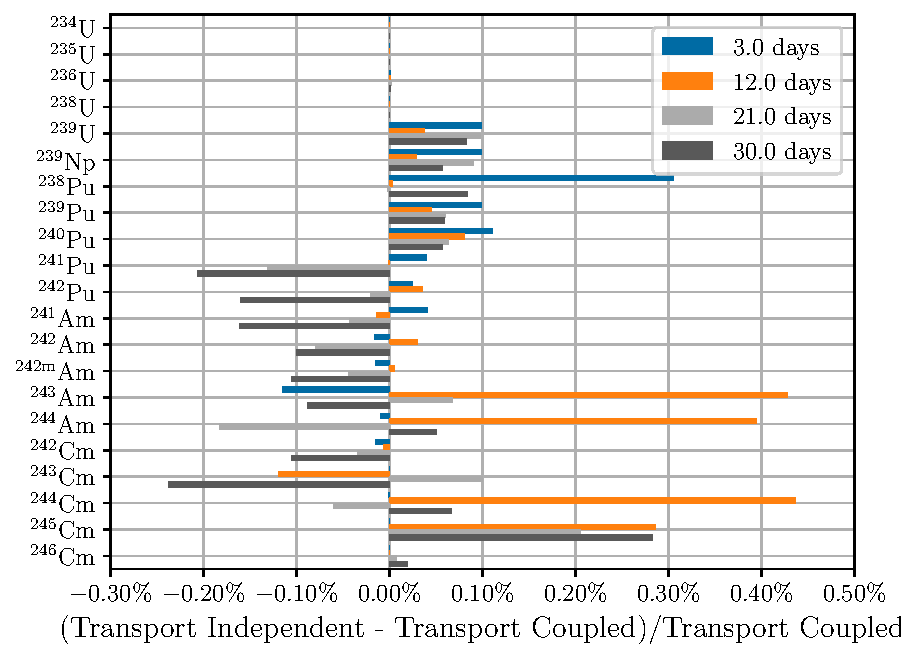
\includegraphics[width=\linewidth]{figs/actinides_updating_xs_predictor_fission_q_days.pdf}
        \caption[]{Actinide error in the fuel using updating cross sections}
        \label{fig:actinides-error-updating-xs}
    \end{figure}
    
    We suspect that the errors for isotopes of \ce{Am} and \ce{Cm} are so high
    are due to their extremely low composition in the fuel.
    %expand on this?


    % fission products error

    \begin{figure}[h!tpb]
        \centering
        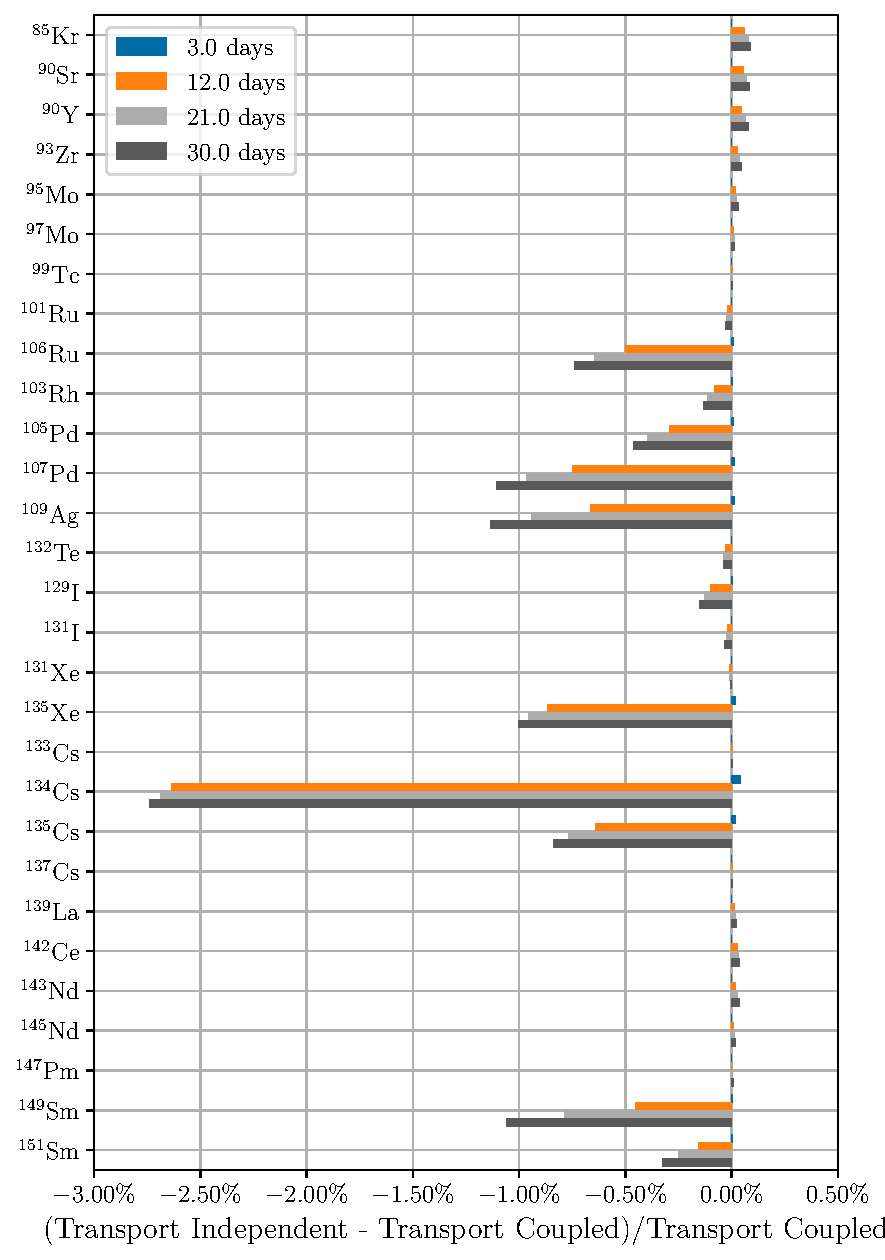
\includegraphics[width=\linewidth]{figs/fission_products_constant_xs_predictor_fission_q_days.pdf}
        \caption{Fission product error using constant cross sections}
        \label{fig:fp-error-constant-xs}
    \end{figure}

    Figures \ref{fig:fp-error-constant-xs} and \ref{fig:fp-error-updating-xs}
    show the relative error for fission products using constant cross sections
    and updating cross sections, respectively.

    Similar to the actinides, updating the cross sections at each depletion step
    results in errors in the nuclide compositions  that are fractions of
    percents. However, unlike the actinides, the errors when using constant
    cross sections are all relavtively low, with the largest error being under
    3\%. A majority of our fissile material is uranium, specifically
    \ce{^{235}U}, and the error for that nuclide is so low that it doesn't even
    show on Figure \ref{fig:actinides-error-constant-xs}. It follows that the
    majority of our fission products come from \ce{^{235}U} in a composition
    that is equally low in error. The other actinides are present in amounts
    with higher error, but in very low quantities, so their effect on the error
    of the fission product compoistions is proportionaly small.
    
    \begin{figure}[htpb]
        \centering
        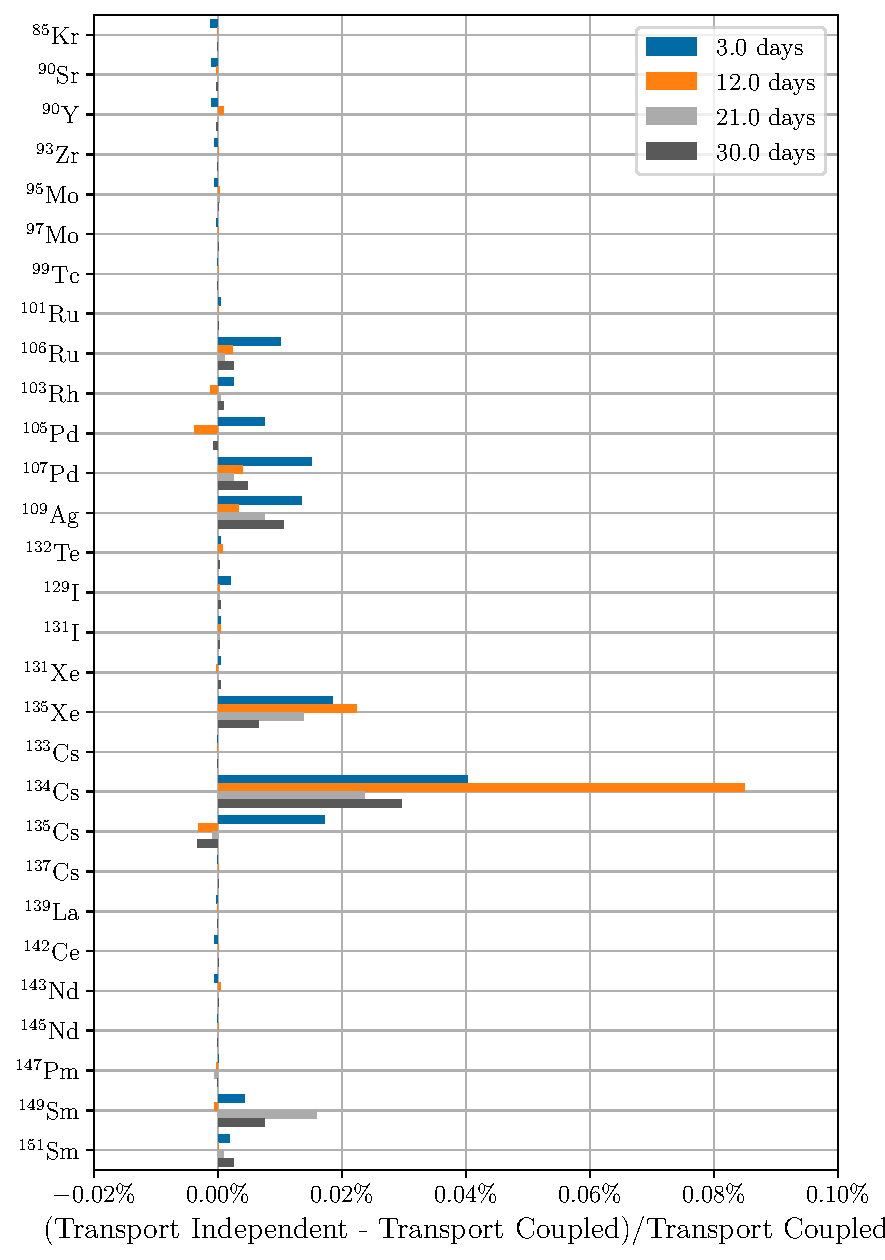
\includegraphics[width=\linewidth]{figs/fission_products_updating_xs_predictor_fission_q_days.pdf}
        \caption{Fission product error using  updating cross sections}
        \label{fig:fp-error-updating-xs}
    \end{figure}

    \begin{figure}[htpb]
        \centering
        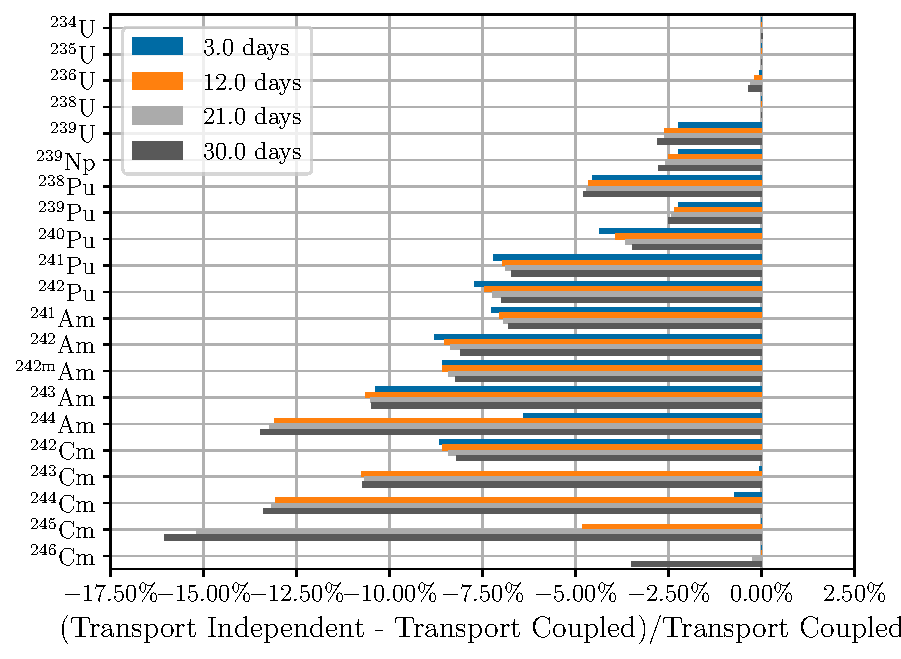
\includegraphics[width=\linewidth]{figs/actinides_constant_xs_cecm_fission_q_days.pdf}
        \caption{Actinide error using the CECM integrator}
        \label{fig:actinides-error-cecm}
    \end{figure}


    % actinides predictor vs cecm
    Figure \ref{fig:actinides-error-cecm} shows the error for actinides using the
    \verb.CECM. integrator. Comparing these results with those of Figure
    \ref{fig:actinides-error-constant-xs} we do not see a significant difference
    in the error. For certain nuclides, the \verb.CECM. integrator appears to
    perform worse. We see a similar pattern for the fission products.

    \begin{figure}[htpb]
        \centering
        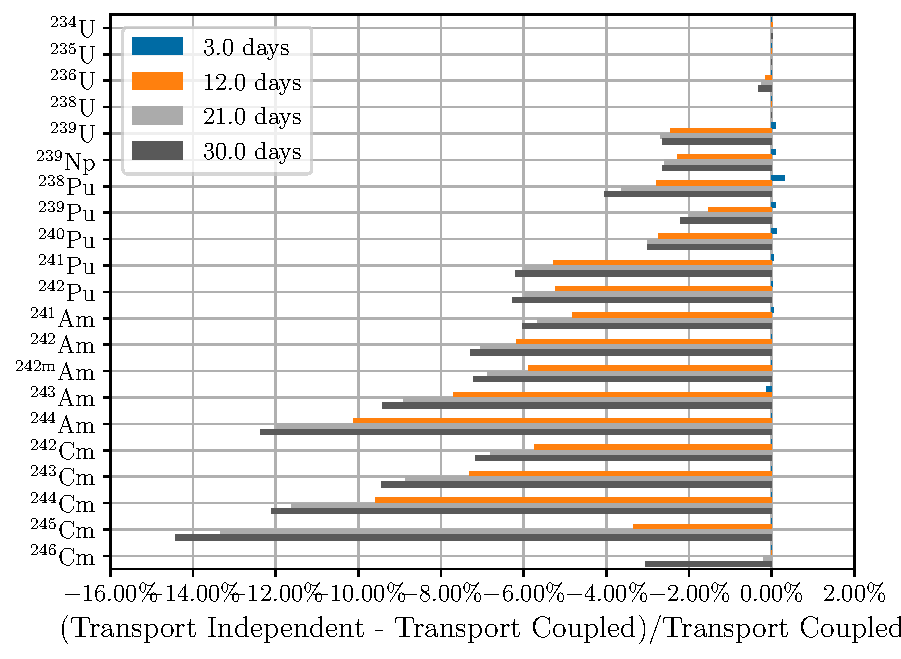
\includegraphics[width=\linewidth]{figs/actinides_constant_xs_predictor_source_rate_days.pdf}
        \caption{Actinide error using explicit value for the flux}
        \label{fig:actinides-error-source}
    \end{figure}

    Figure \ref{fig:actinides-error-source} shows the error for actinides using
    the flux we calculated from the initial material composition. These results
    do not differ significantly from the results in Figure
    \ref{fig:actinides-error-constant-xs}. The same is true for the fission
    products.

    Finally, a word on runtime; unfortunately, a bug present in the code during
    our study prevented collection of exact runtimes that would normally be
    stored in the statepoint files. Based on our time developing and testing
    this code, as well as running the simulations, the time savings when using
    \verb.IndependentOperator. are immense. Whereas the transport-coupled
    simulations each took several hours to complete, the transport-independent
    simulations took seconds to minutes to complete!

\section{Conclusions}\label{sec:conclusion}
    In this paper, we introduced a new method for running depletion simulations
    in OpenMC. This method relies on pre-calclated one-group cross sections
    stored in a table. The new method is siginifcantly faster than running a
    transport-coupled depletion simulation, albiet with a penalty to accuracy.
    Better accuracy will be obtained in simulations where the neutron flux
    spectrum will be constant, i.e. in fusion simulations.
    
    The geometry used in this study was a simple PWR pincell. We are unsure how
    the method performs with more complex geometries. Future work could
    focus on exploring this.
     
    Currently, we do not have capabilities to calculate $k_\text{eff}$ using
    \verb.IndependentOperator.. We have looked at a implementing a method
    similar to one in  \cite{LOVECKY2014333}, wherein ... (adapt discussion from
    GH issue)

    Finally, while the current method is limited to using one-group cross
    sections, it would not be too difficult to add support for multi-group cross
    sections. The authors estimate that adding support for multiple energy
    groups may increase the accuracy of depletion simulations using
    \verb.IndependentOperator. compared to transport-coupled simulations,
    expecially for more complex geometries.
% Numbered list
% Use the style of numbering in square brackets.
% If nothing is used, default style will be taken.
%\begin{enumerate}[a)]
%\item 
%\item 
%\item 
%\end{enumerate}  

% Unnumbered list
%\begin{itemize}
%\item 
%\item 
%\item 
%\end{itemize}  

% Description list
%\begin{description}
%\item[]
%\item[] 
%\item[] 
%\end{description}  

% Figure
%\begin{figure}[<options>]
%	\centering
%		\includegraphics[<options>]{}
%	  \caption{}\label{fig1}
%\end{figure}


%\begin{table}[<options>]
%\caption{}\label{tbl1}
%\begin{tabular*}{\tblwidth}{@{}LL@{}}
%\toprule
%  &  \\ % Table header row
%\midrule
% & \\
% & \\
% & \\
% & \\
%\bottomrule
%\end{tabular*}
%\end{table}

% Uncomment and use as the case may be
%\begin{theorem} 
%\end{theorem}

% Uncomment and use as the case may be
%\begin{lemma} 
%\end{lemma}

%% The Appendices part is started with the command \appendix;
%% appendix sections are then done as normal sections
%% \appendix

% To print the credit authorship contribution details
\printcredits

%% Loading bibliography style file
%\bibliographystyle{model1-num-names}
\bibliographystyle{cas-model2-names}

% Loading bibliography database
\bibliography{bibliography}

% Biography
%\bio{}
% Here goes the biography details.
%\endbio

%\bio{pic1}
% Here goes the biography details.
%\endbio

\end{document}

